\documentclass{beamer}
\usetheme{Boadilla}
\usepackage[utf8]{inputenc}

\usepackage{amsmath, amsthm}
\usepackage{bm}
\usepackage{tikz}
\usepackage{graphicx}
\usepackage{listings}
\usepackage{tcolorbox, transparent}
\usepackage[abs]{overpic}
\usepackage{color}
\definecolor{bn}{HTML}{F2300F}
\definecolor{an}{HTML}{0B775E}
%\usepackage{hyperref}
%\hypersetup{urlcolor=blue, colorlinks=true} 
%\usetikzlibrary{positioning, spy, calc}
%\usetikzlibrary{decorations.markings}
\def\norm#1{\left|\left|#1\right|\right|} 
\def\rbr#1{\left(#1\right)} 
\def\bR{\mathbb{R}}
\def\arrA{\mathcal{A}}
\def\arrB{\mathcal{B}}
\def\eps{\varepsilon}
\DeclareMathOperator{\rank}{rank}
\usepackage[
backend=biber,
style=alphabetic,
sorting=ynt
]{biblatex}

\addbibresource{mybib.bib}

\title[COVID-19 Modelling]{
Modelling the Spread of COVID-19 Cases}
\subtitle{MAU44M00: Mathematics Project Presentation}
\author[Anthony Gibbons]{\textbf{Anthony Gibbons} \\
Student number: 17322353 \\
\textbf{Supervisor: Athanasios Georgiadis}}
\date{February 2021}

\begin{document}

\begin{frame}
\titlepage
\end{frame}

\begin{frame}
The Coronavirus disease (COVID-19) was first characterized by the World Health Organisation as pandemic on 11th March 2020. The outbreak has affected almost every aspect of human life throughout 2020, and is expected to continue for much of 2021.
\end{frame}

\begin{frame}{Daily Cases Worldwide \cite{countrydata}}
\begin{figure}[H]
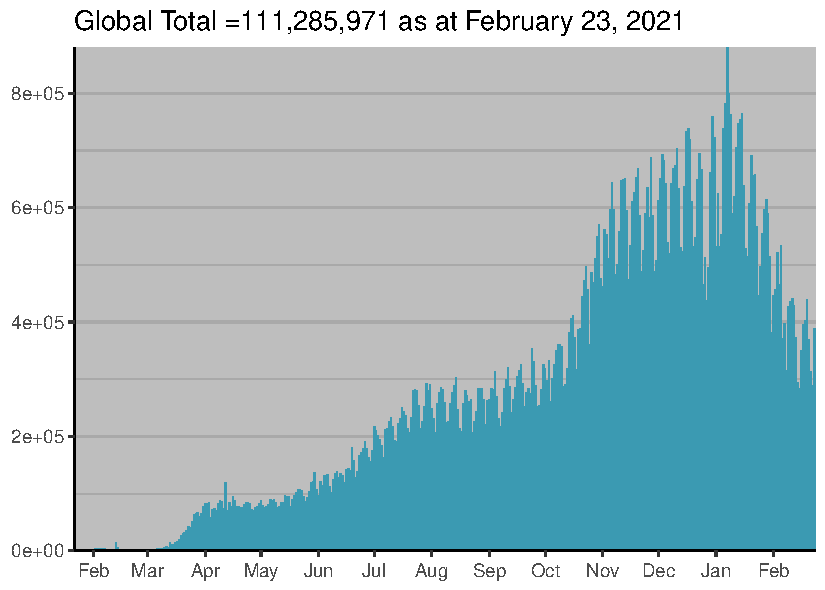
\includegraphics[width=0.9\textwidth]{Plots/WorldTotal-xn.pdf}
\end{figure}
\end{frame}

\begin{frame}{Situation in Ireland \cite{irelanddata}}
\begin{figure}
\centering
\minipage{0.49\textwidth}
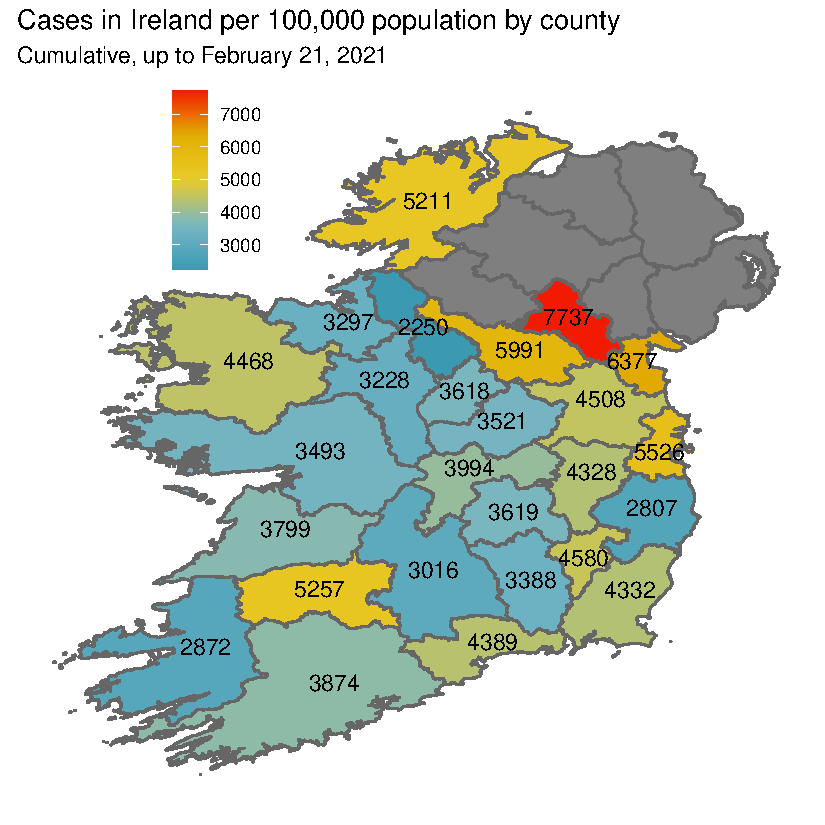
\includegraphics[width=0.9\textwidth]{Plots/county-rep.pdf}
\endminipage\hfill
\minipage{0.49\textwidth}
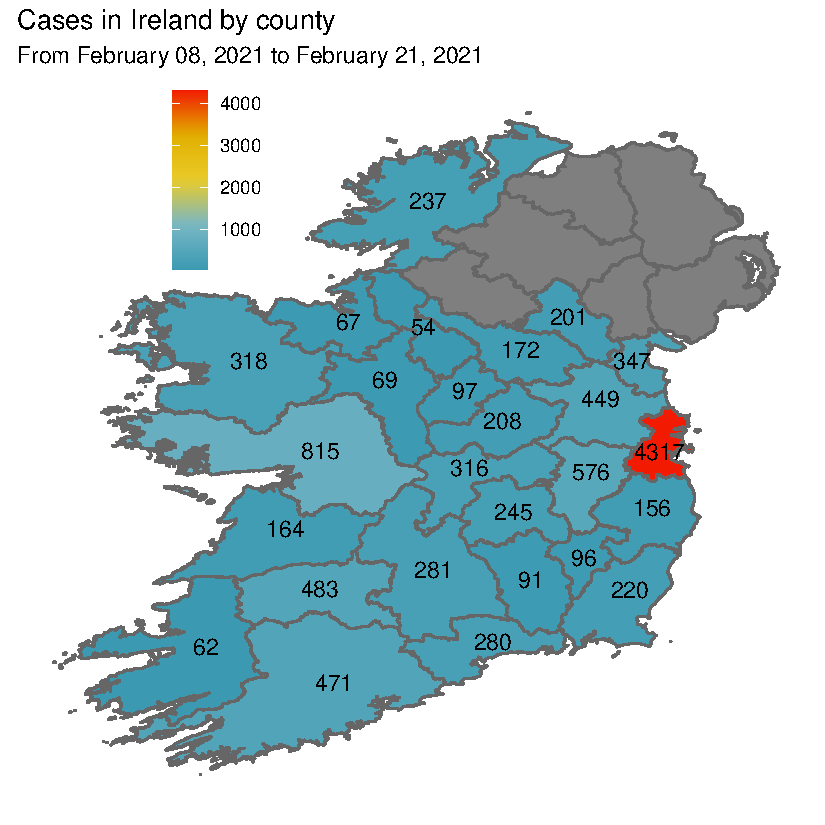
\includegraphics[width=0.9\textwidth]{Plots/county-fourteendaycases.pdf}
\endminipage
\end{figure}
\end{frame}

\begin{frame}{Basic Model - Assumptions \cite{grigor20}}
    \begin{itemize}
    \item[(I)] Any infected person becomes ill (symptomatic) and infectious on the $q$-th day after infection.\footnote{The number of days before an infected person becomes infectious is called the latent period, and before he/she becomes symptomatically ill – the incubation period. Here we assume for simplicity that these two periods are equal.}
    \item[(A)] During each day, each ill person unconfined infects on average $a$ other persons.
    \item[(B)] During each day, a fraction $b$ of ill people loose gets isolated (hospitalized or otherwise) and withdrawn from a further spread of the epidemic.
\end{itemize}
\end{frame}

\begin{frame}{Basic Model - Implementation}
$x_n^*$ is the actual number of reported cases on day $n$

$x_n$ is the (according to the model) number of infected people that are detected and isolated during the day $n$

\begin{equation*} \label{eq:xnrecurr}
    x_{n+1} = (1 - b) x_n + ax_{n-q}.
\end{equation*}

We let the model equal the actual data for the first $q+1$ days
\begin{equation*} \label{eq:xn0q}
x_n = x^*_n \ \text{for} \ n = 0, 1, \dots , q,
\end{equation*}

 To fit our model we optimize against the normalized 1-norm:
\begin{equation*}\label{eq:xnnorm}
    \norm{x^*-x}:= \frac{1}{N+1} \sum\limits_{n=0}^N |x_n-x_n^*|.
\end{equation*}
\end{frame}

\begin{frame}{United States - Basic Model}
\begin{figure}
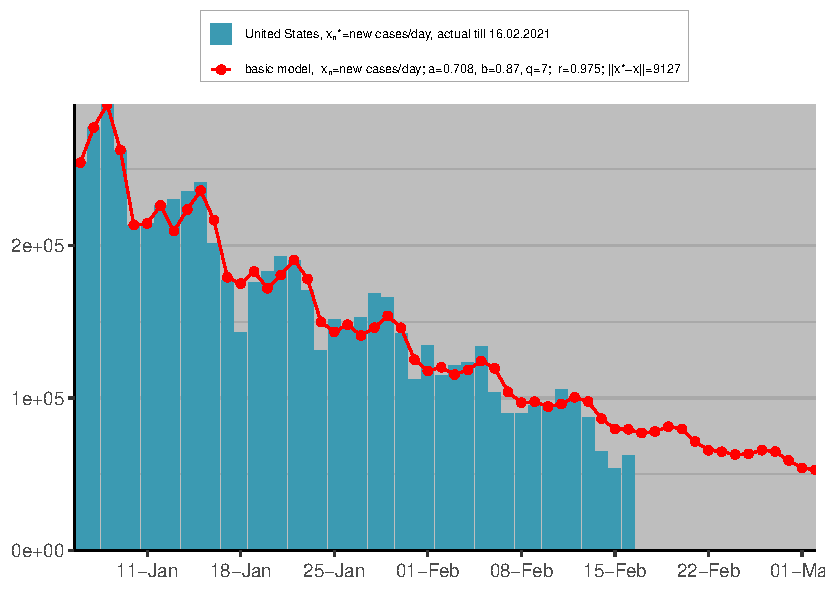
\includegraphics[width=0.9\textwidth]{Plots/United States-basexn.pdf}
\end{figure}
\end{frame}

\begin{frame}{United States - Basic Model}
\begin{figure}
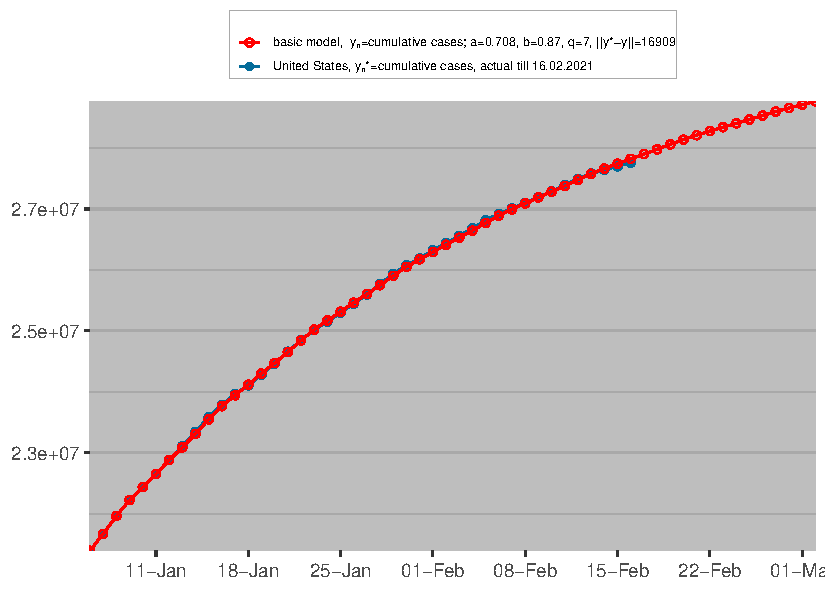
\includegraphics[width=0.9\textwidth]{Plots/United States-baseyn.pdf}
\end{figure}
\end{frame}

\begin{frame}{United States - Limiting Curve}
\begin{figure}
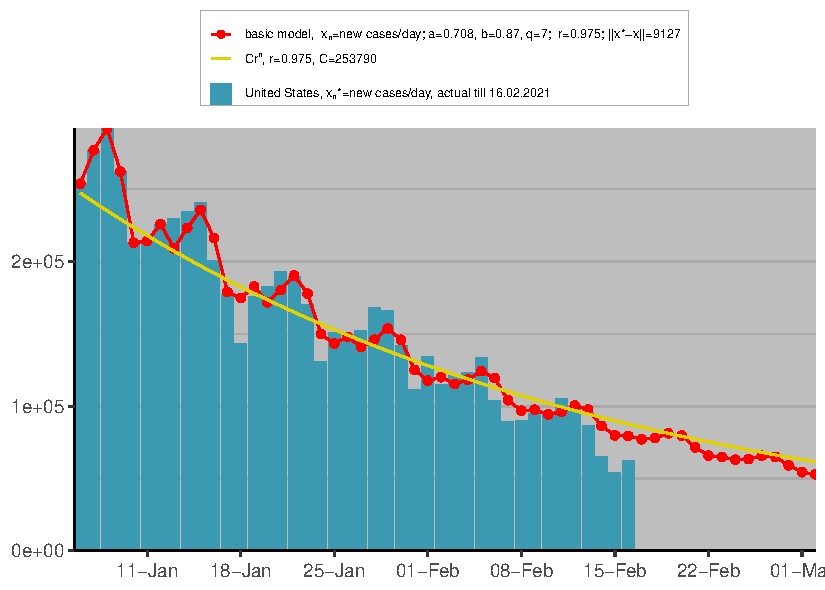
\includegraphics[width=0.9\textwidth]{Plots/United States-Crn.pdf}
\end{figure}
\end{frame}

\begin{frame}{Ireland - Limiting Curve Growing Exponentially}
\begin{figure}
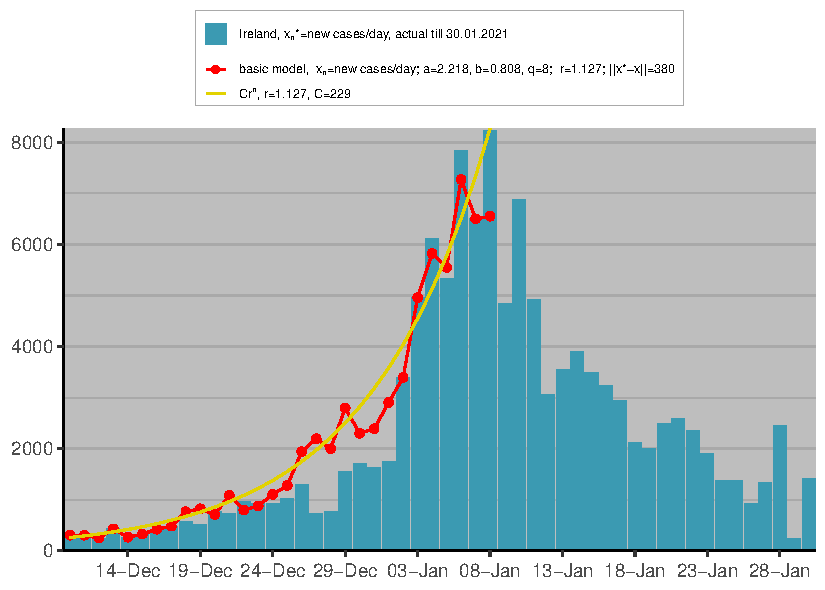
\includegraphics[width=0.9\textwidth]{Plots/Ireland-expgrowth.pdf}
\end{figure}
\end{frame}

\begin{frame}{United States - Periodic Parameters}
\begin{overpic}[unit=1mm,tics=10,width=0.9\linewidth]{Plots/United States-perparam.pdf}
    \put(60,35){%
      \makebox[0pt]{%
        \transparent{0}%
        \colorbox[rgb]{0,0,1}{%
          \parbox[b]{9cm}{%
            \transparent{1}%
            \color{bn}{
            $b_n := b\rbr{1+c_2\rbr{\sin\rbr{\frac{2\pi}{p_2}\rbr{n-n_2}}}}$}
            
            \vspace{1ex}
            \color{an}{
            $a_n := a\rbr{1+c_1\rbr{\sin\rbr{\frac{2\pi}{p_1}\rbr{n-n_1}}}}$}
          }%
        }%
      }%
    }%
  \end{overpic}
%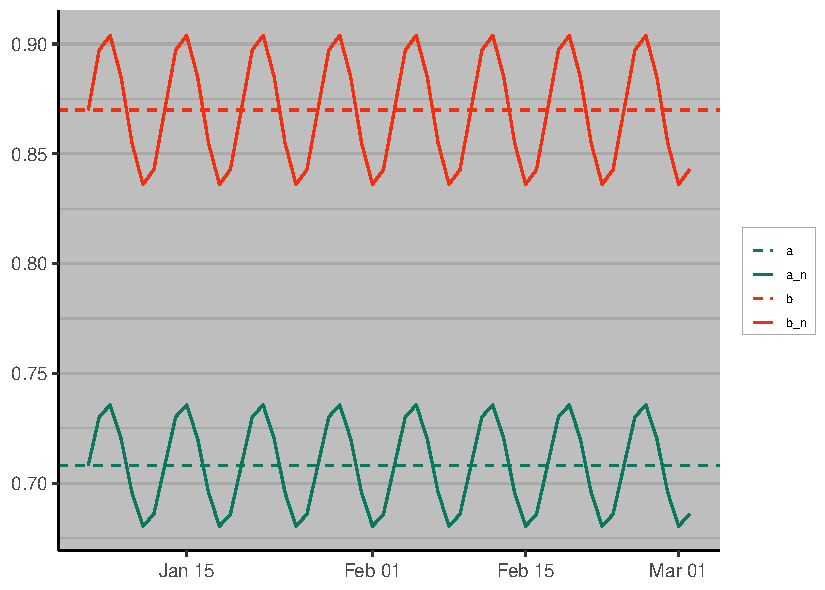
\includegraphics[width=0.9\textwidth]{Plots/United States-perparam.pdf}
\end{frame}

\begin{frame}{United States - Periodic Model}
\begin{figure}
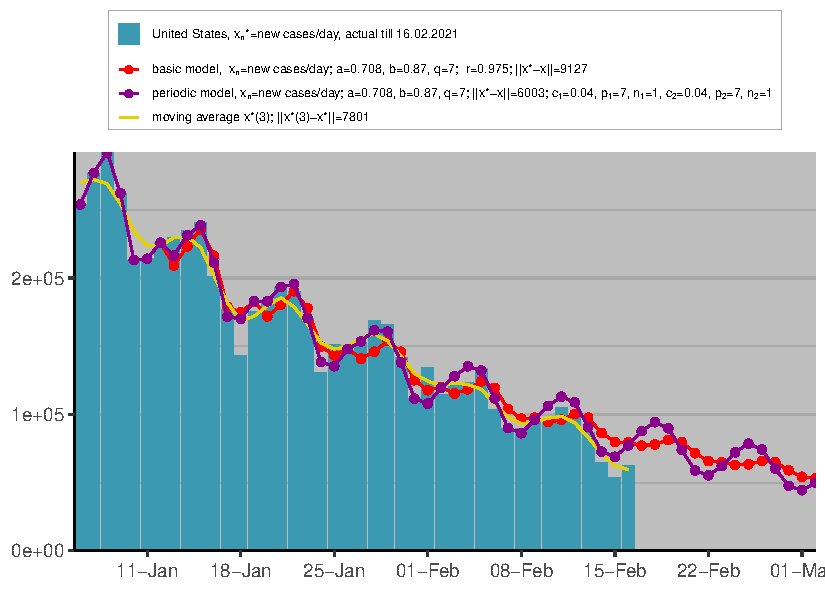
\includegraphics[width=0.9\textwidth]{Plots/United States-periodic.pdf}
\end{figure}
\end{frame}

%\begin{frame}{Ireland - Multi-phase periodic model}
%\begin{figure}
%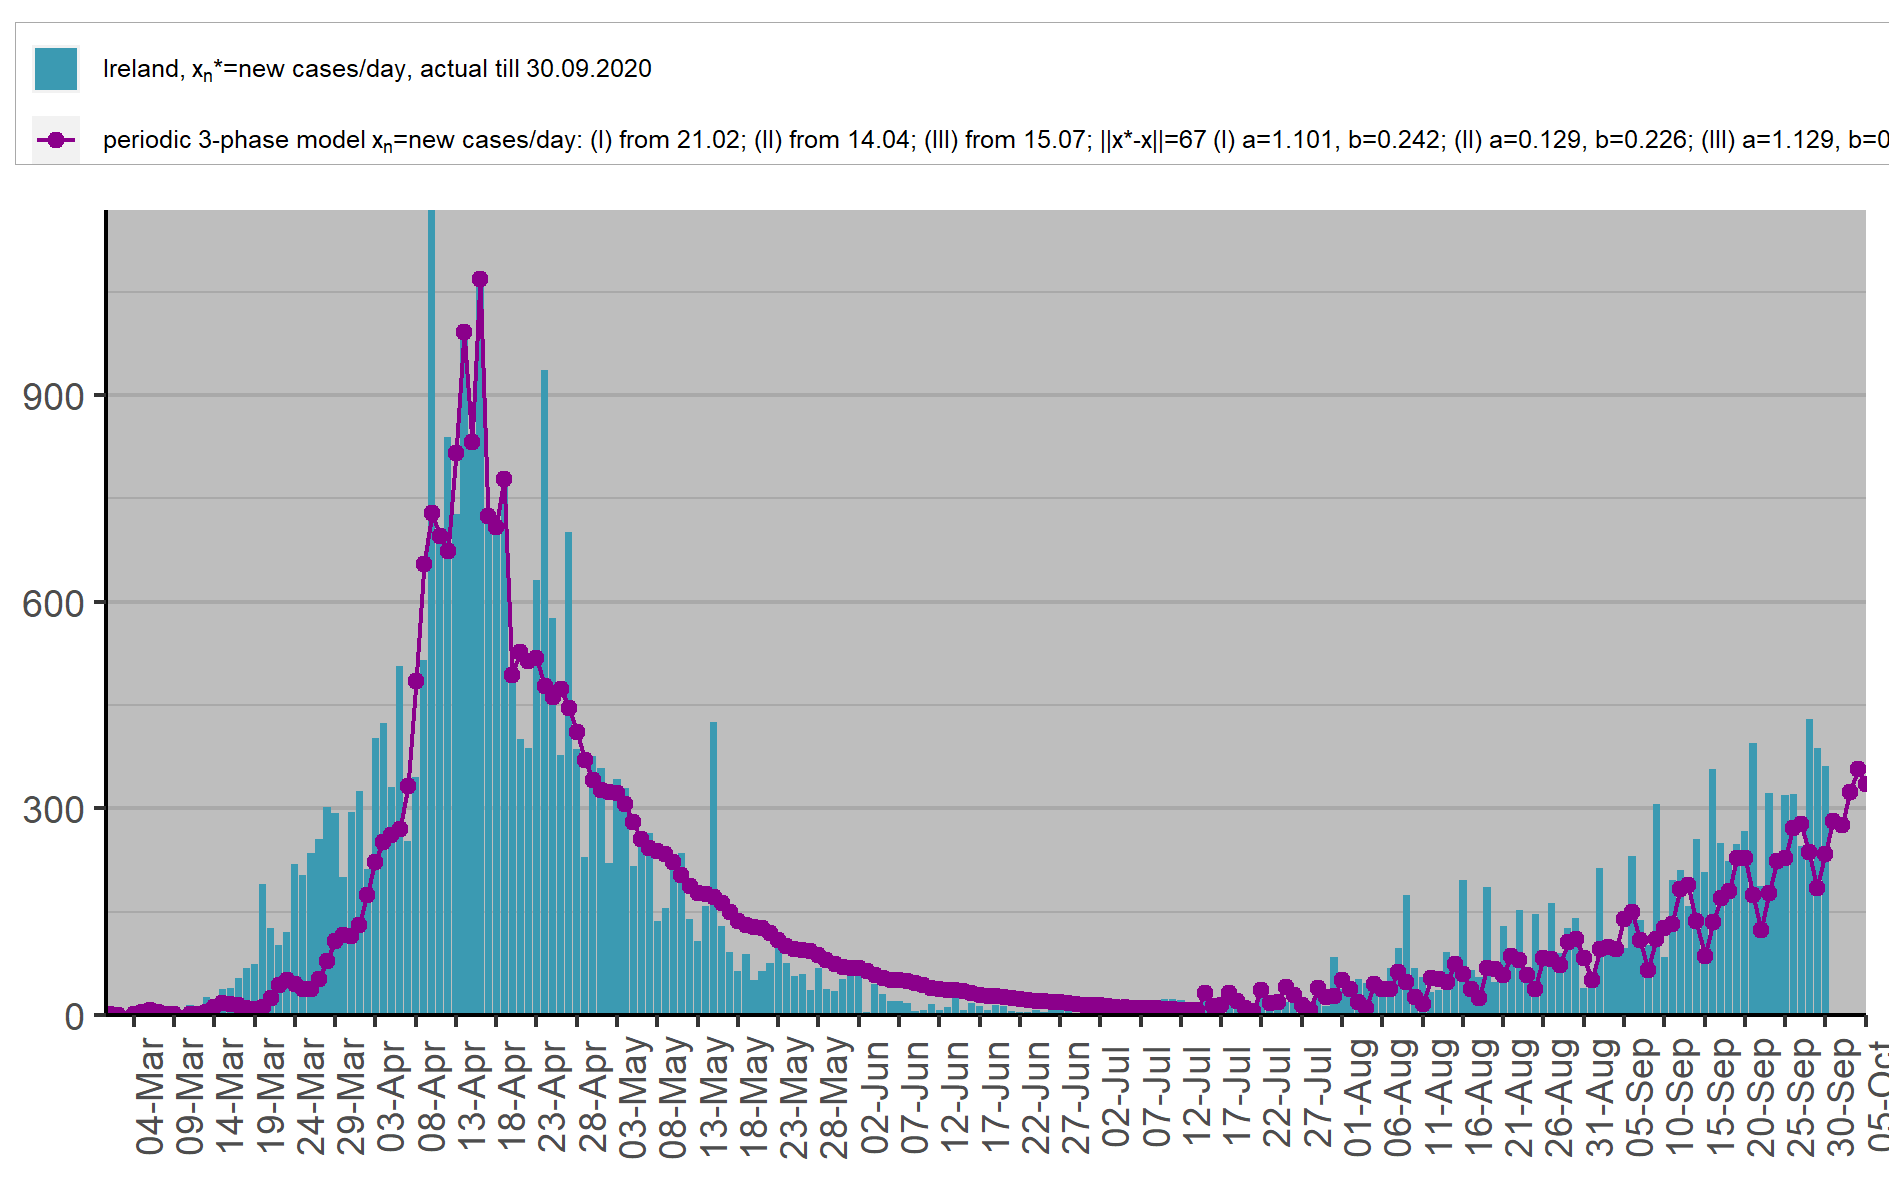
\includegraphics[width=0.9\textwidth]{Plots/Ireland-perxnmult.png}
%\end{figure}
%\end{frame}

%\begin{frame}{Ireland - Multi-phase periodic model}
%\begin{figure}
%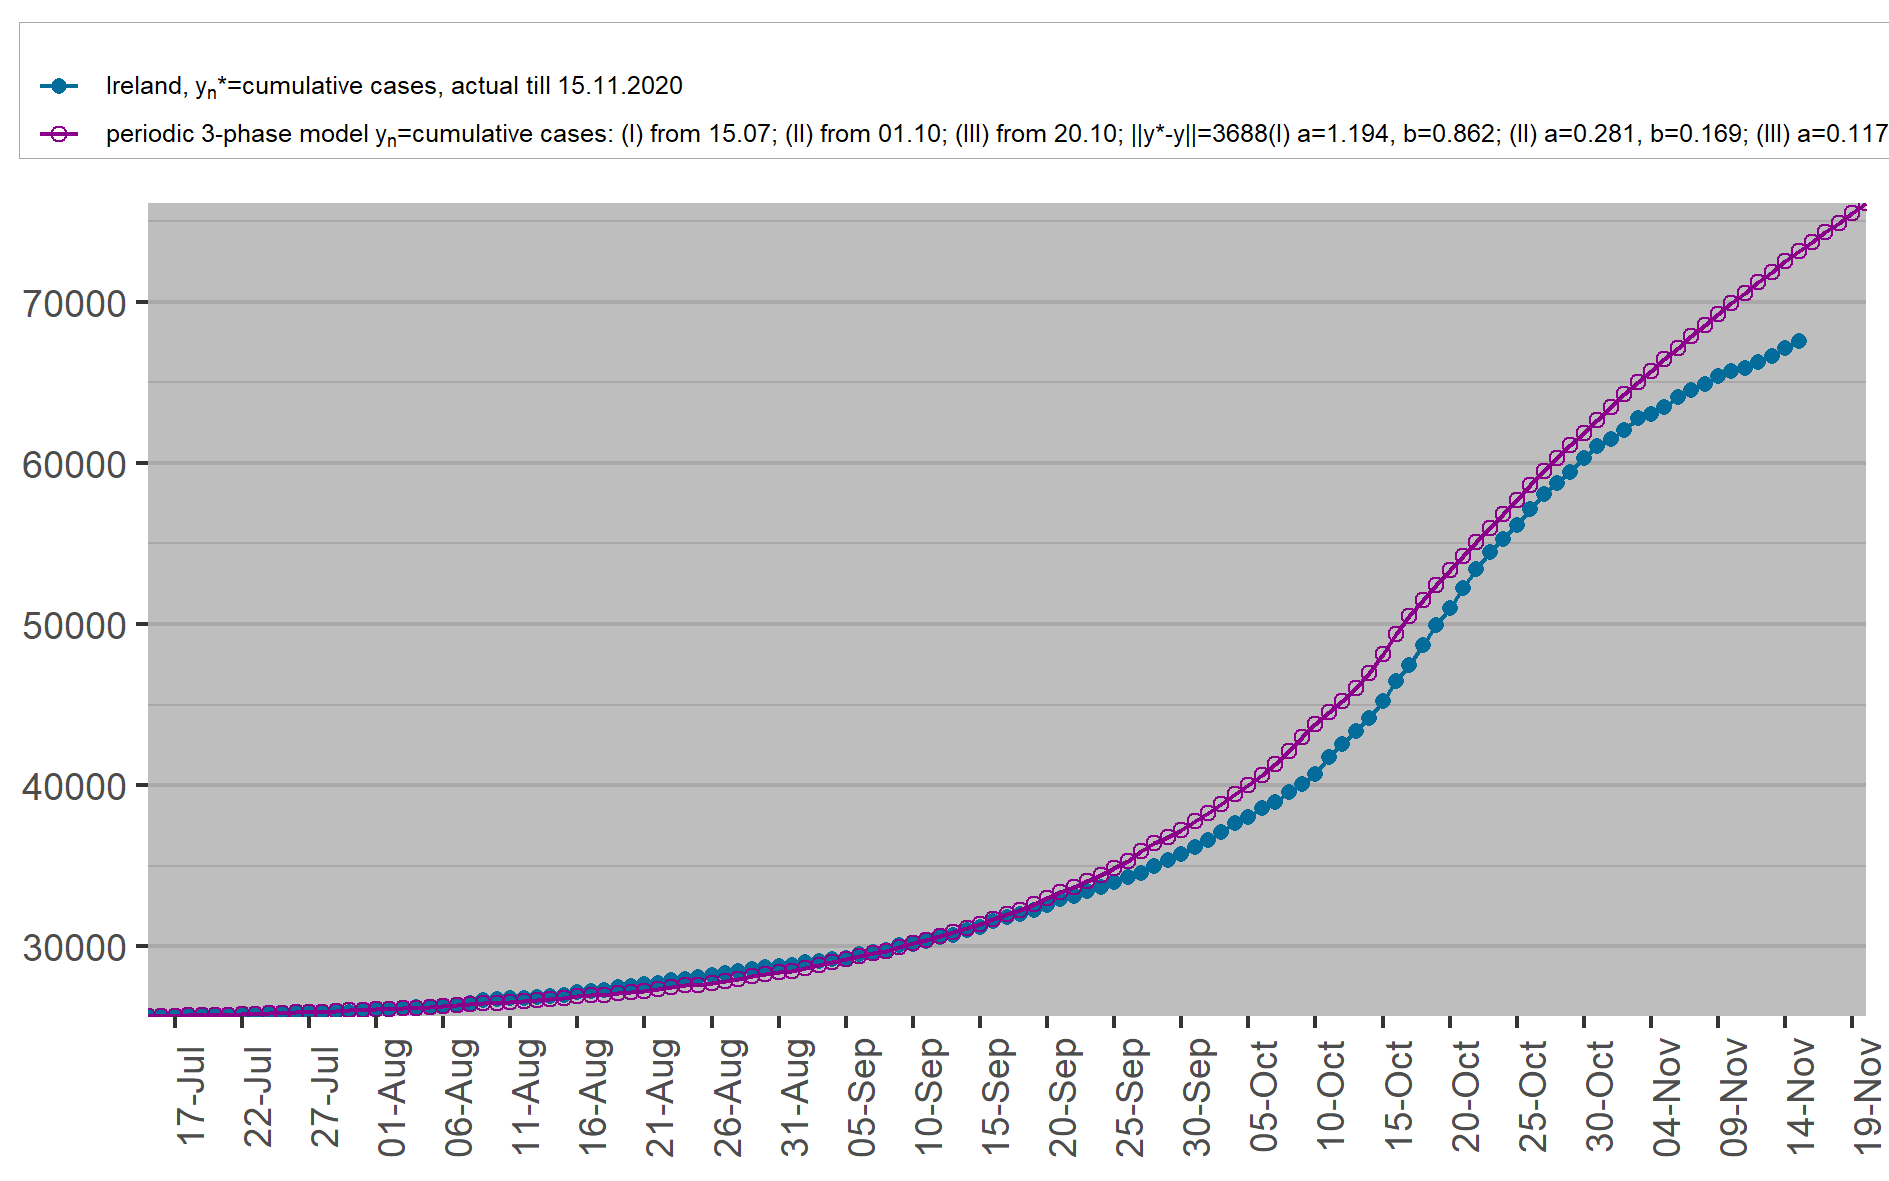
\includegraphics[width=0.9\textwidth]{Plots/Ireland-perynmult.png}
%\end{figure}
%\end{frame}

\begin{frame}{Time series decomposition \cite{Hyndman-et-al-2018}}
\begin{figure}
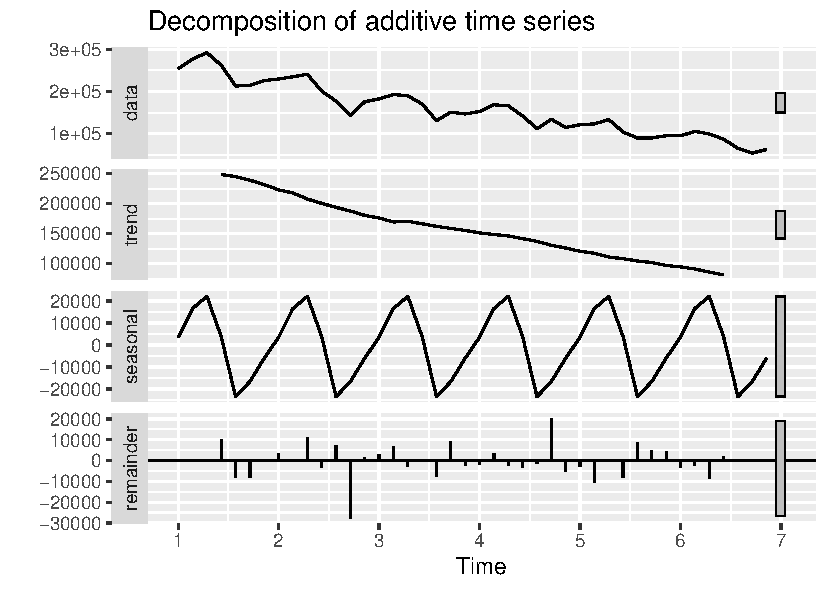
\includegraphics[width=0.9\textwidth]{Plots/United States-tsdecompose.pdf}
\end{figure}
\end{frame}

\begin{frame}{Holt-Winters Model}
\begin{figure}[H]
\begin{tcolorbox}[width=.87\textwidth]%

Suppose there are $N$ observations.

Initial step:

$\left|\begin{array}{l}
L_s = \frac1s \sum_{i=1}^s x_i \\
b_s = \frac1s \left[\frac{x_{s+1}-x_1}{s}+\frac{x_{s+2}-x_2}{s}+\dots+\frac{x_{2s}-x_s}{s}\right]\\
S_n  = x_n-L_s, \ n=1,\dots,s
\end{array}\right.$

and choose parameters $0\leq\alpha,\beta,\gamma\leq1$

Then compute for $s<n\leq N$:

$\left|\begin{array}{lll}
\text{Level} &       L_n & = \alpha (x_n-S_{n-s})+(1-\alpha)(L_{n-1}+b_{n-1})\\
\text{Trend} &      b_n & = \beta(L_n-L_{n-1})+(1-\beta)b_{n-1}\\
\text{Seasonal} & S_n & = \gamma (x_n-L_n) + (1-\gamma)S_{n-s}\\
\text{Forecast} & F_{n+1} & = L_n+b_n+S_{n+1-s}
\end{array}\right.$
For subsequent observations,

$F_{N+k}=L_N+k\cdot b_N+S_{N+k-s}$
\label{SHWx}
\end{tcolorbox}
\caption{Seasonal Holt Winter’s Additive Model Algorithm (denoted SHW$_{+}$)}
\end{figure}
\end{frame}

\begin{frame}{United States - Holt-Winters Model}
\begin{figure}
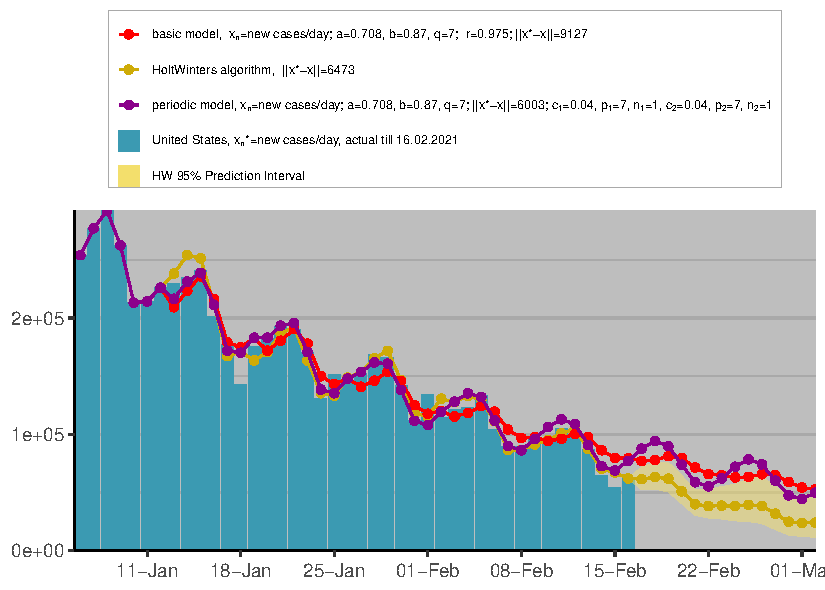
\includegraphics[width=0.9\textwidth]{Plots/United States-hw.pdf}
\end{figure}
\end{frame}

\begin{frame}{United States - Holt-Winters Model}
\begin{figure}
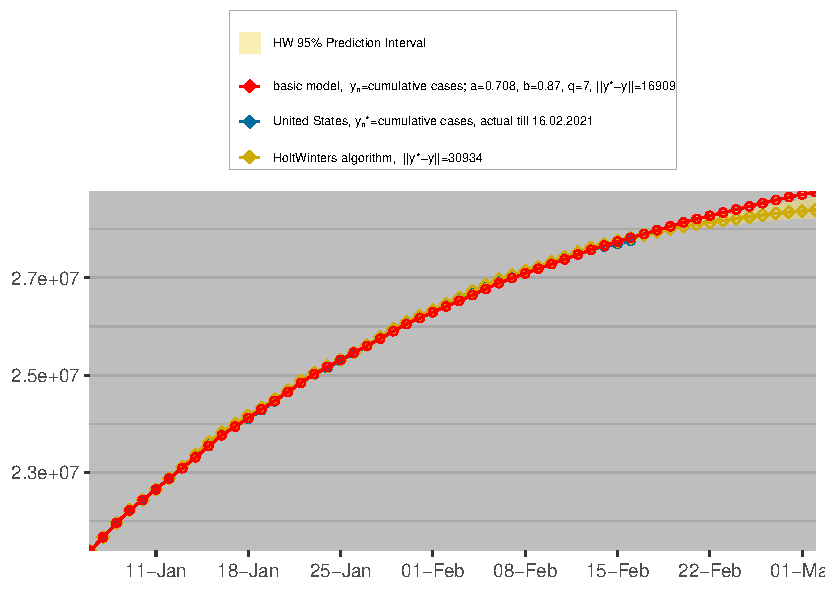
\includegraphics[width=0.9\textwidth]{Plots/United States-hwy.pdf}
\end{figure}
\end{frame}

\begin{frame}{ARIMA$(p,d,q)$ Model}
  A non-seasonal AutoRegressive Integrated Moving Average Model is defined as
  
\begin{align}
\underbrace{\left(1-\phi_1 B-\phi_2B^2-\dots-\phi_p B^p\right)}_{AR(p)}
\underbrace{\left(1-B\right)^d}_{I(d)} x_n = \nonumber \\
 c+
\underbrace{\left(1-\psi_1 B-\psi_2B^2-\dots-\psi_q B^q\right)}_{MA(q)} \eps_n \nonumber
\end{align}

where $B^k x_n = x_{n-k}$

The orders $p,d,q$ are computed by analysing the correlation functions (ACF and PACF).

The $p+q+1$ coefficients $c,\phi_1,\dots,\phi_p,\psi_1,\dots,\psi_q$ are computed using Maximum Likelihood Estimation
\end{frame}

\begin{frame}{United States - ARIMA$(p,d,q)(P,D,Q)$ Model}
\begin{figure}
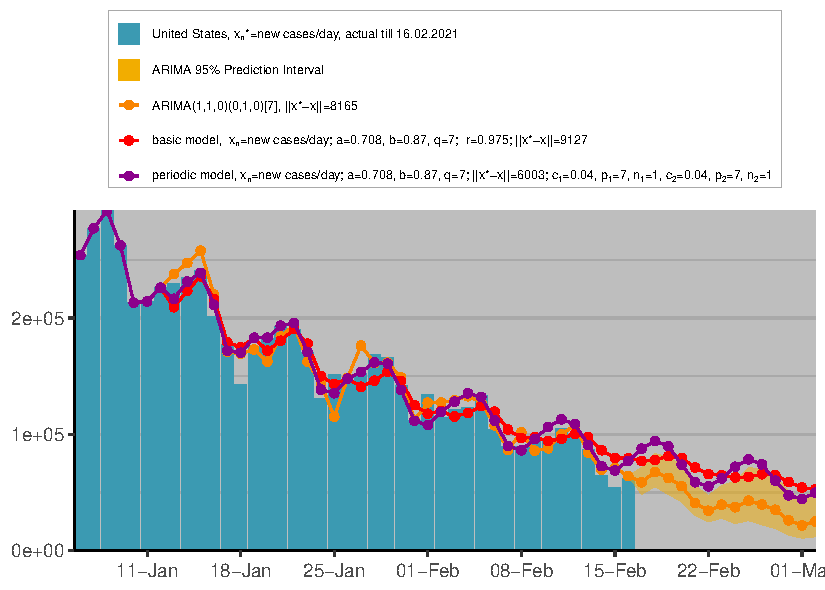
\includegraphics[width=0.9\textwidth]{Plots/United States-arima.pdf}
\end{figure}
\end{frame}

\begin{frame}{United States - ARIMA$(p,d,q)(P,D,Q)$ Model}
\begin{figure}
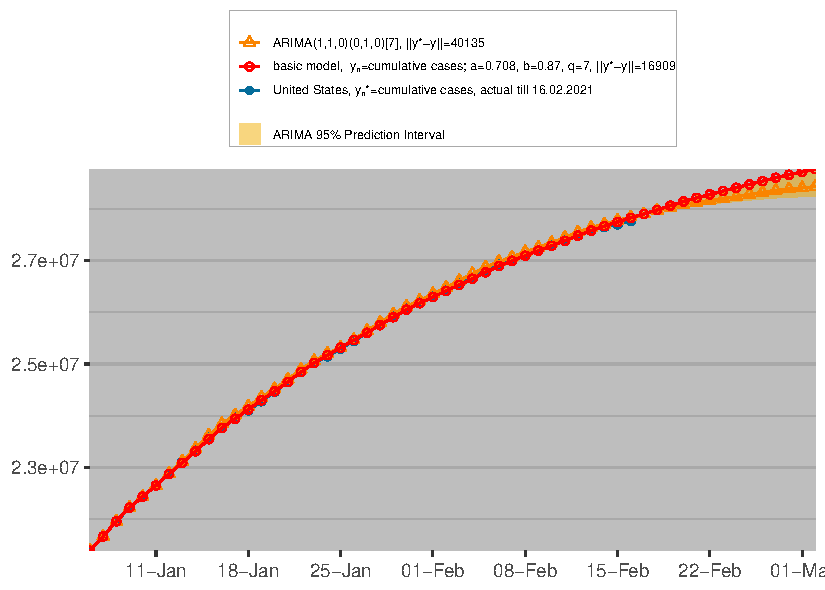
\includegraphics[width=0.9\textwidth]{Plots/United States-arimay.pdf}
\end{figure}
\end{frame}

\begin{frame}{Regression or ARIMA$(p,0,0)$ Model}
\begin{figure}
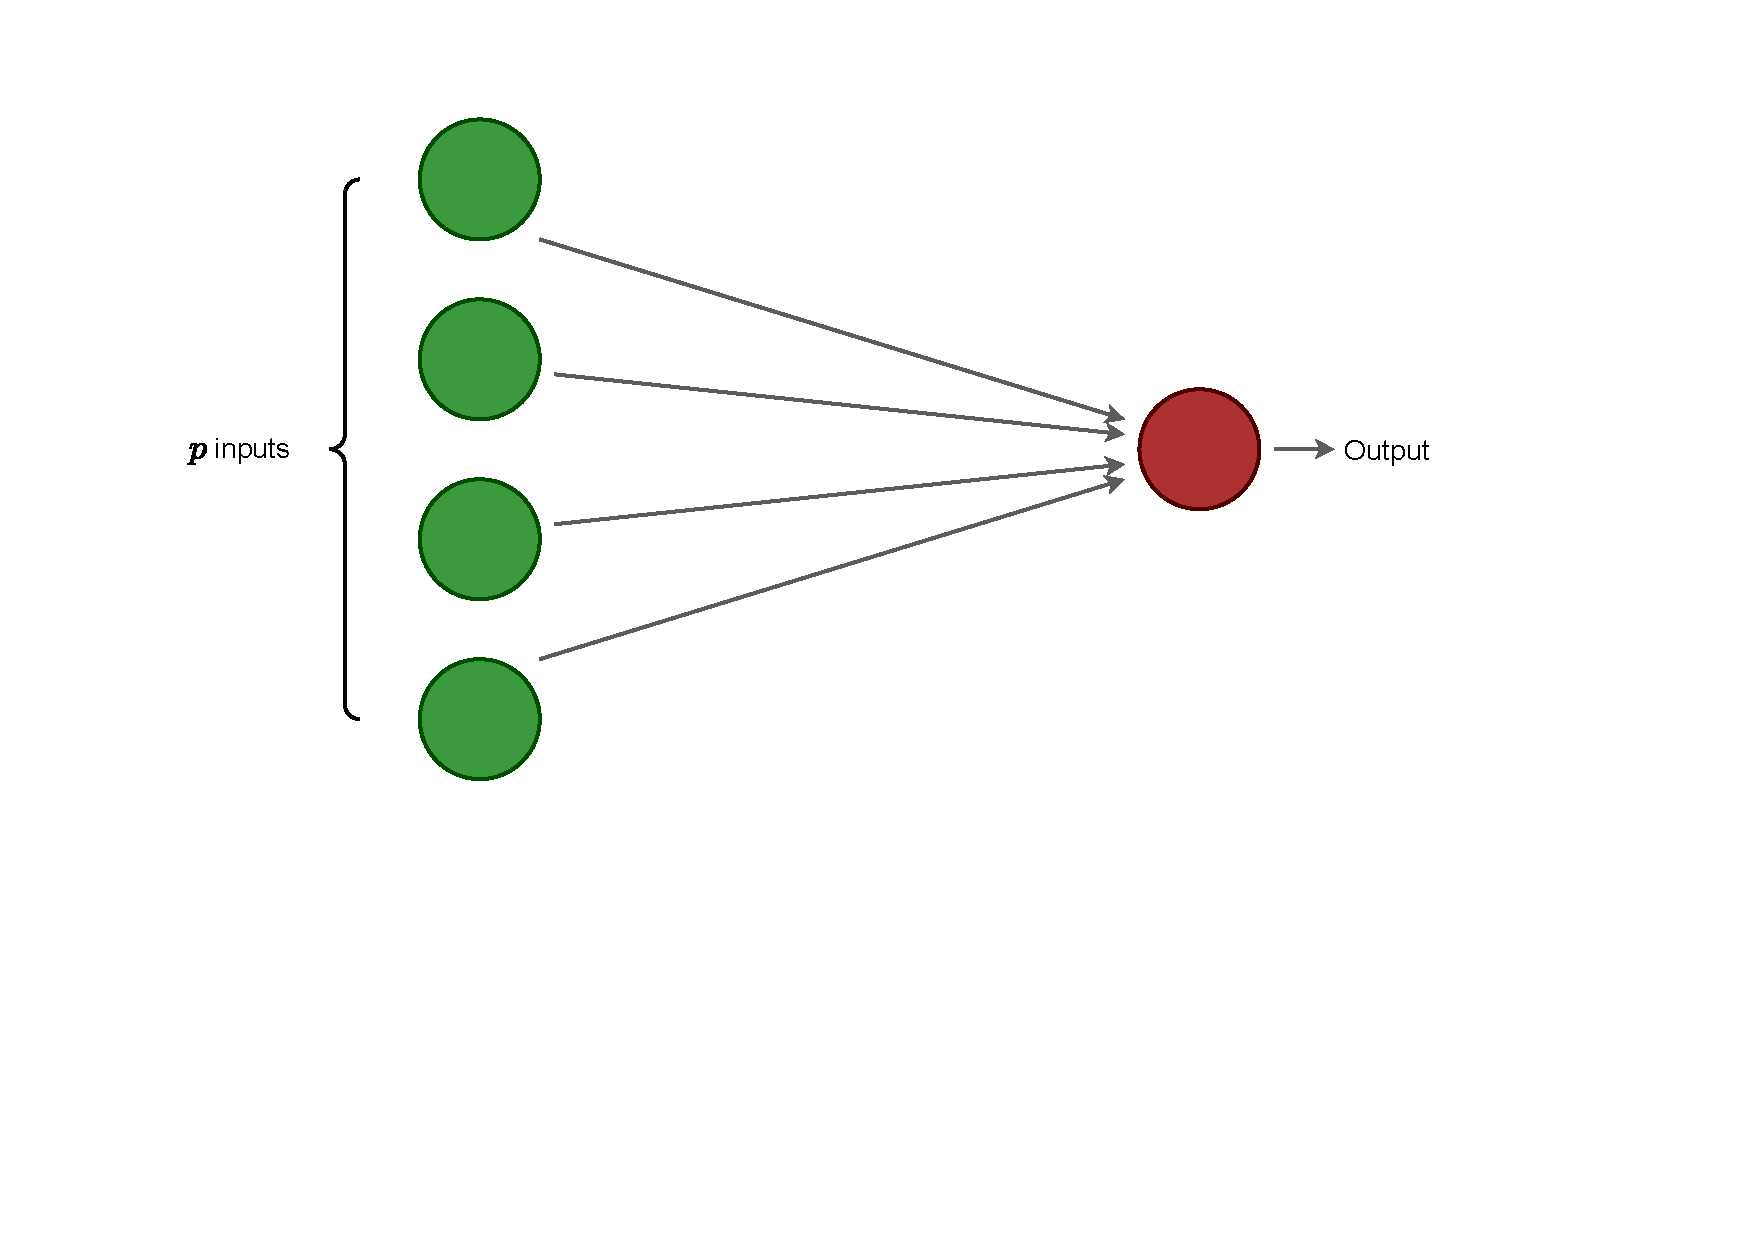
\includegraphics[trim={1cm 6cm 4cm 1cm},clip, width=0.95\textwidth]{Plots/NeuralNetNoHidden.pdf}
\caption{A linear regression model, or ARIMA$(p,0,0)$ model.}
\end{figure}
\end{frame}

\begin{frame}{Neural Network NNAR$(p,k,0)$ Model}
\begin{figure}
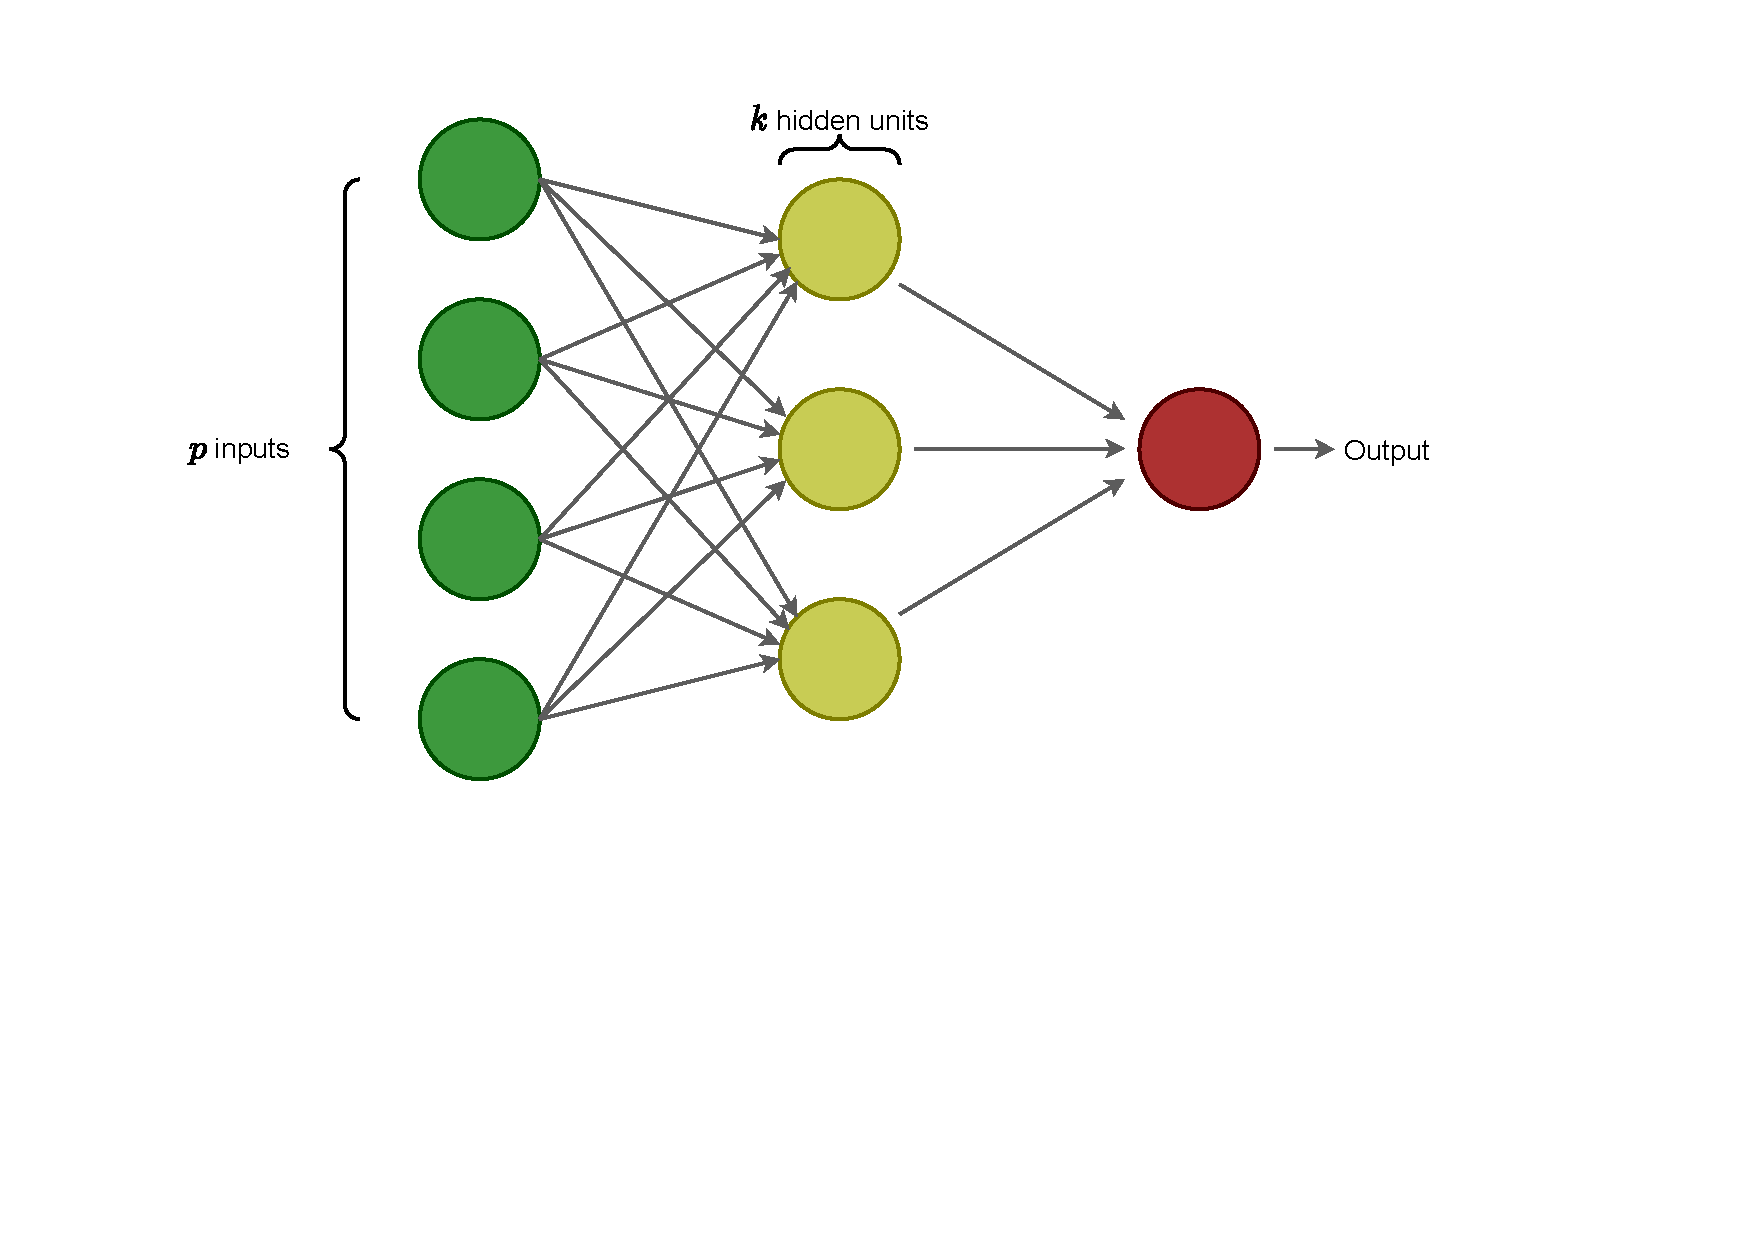
\includegraphics[trim={1cm 6cm 4cm 1cm},clip,, width=0.95\textwidth]{Plots/NeuralNet.pdf}
\caption{A neural network with $p$ inputs and one hidden layer with $k$ hidden neurons.}
\end{figure}
\end{frame}

\begin{frame}{United States - Neural Network Autoregression Model NNAR$(p,k,P)$}
\begin{figure}
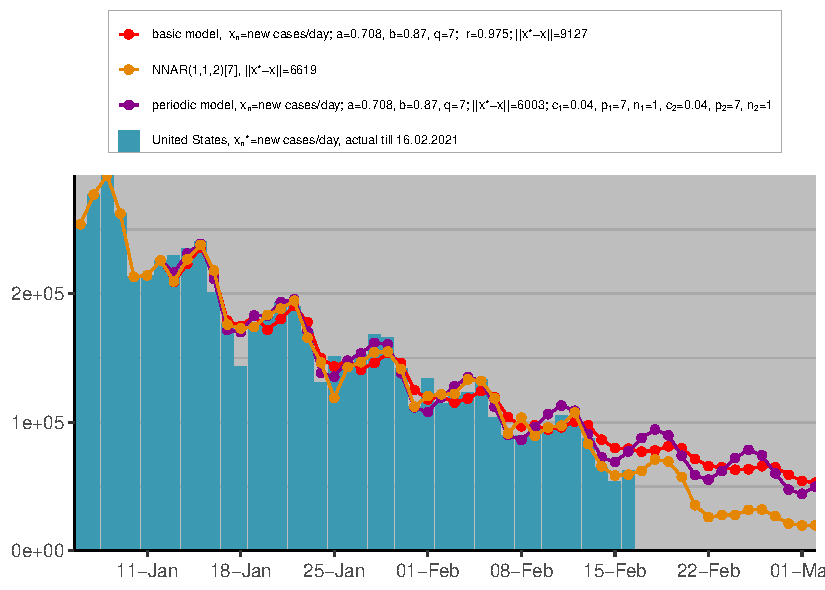
\includegraphics[width=0.9\textwidth]{Plots/United States-nn.pdf}
\end{figure}
\end{frame}

\begin{frame}{United States - Neural Network Autoregression Model NNAR$(p,k,P)$}
\begin{figure}
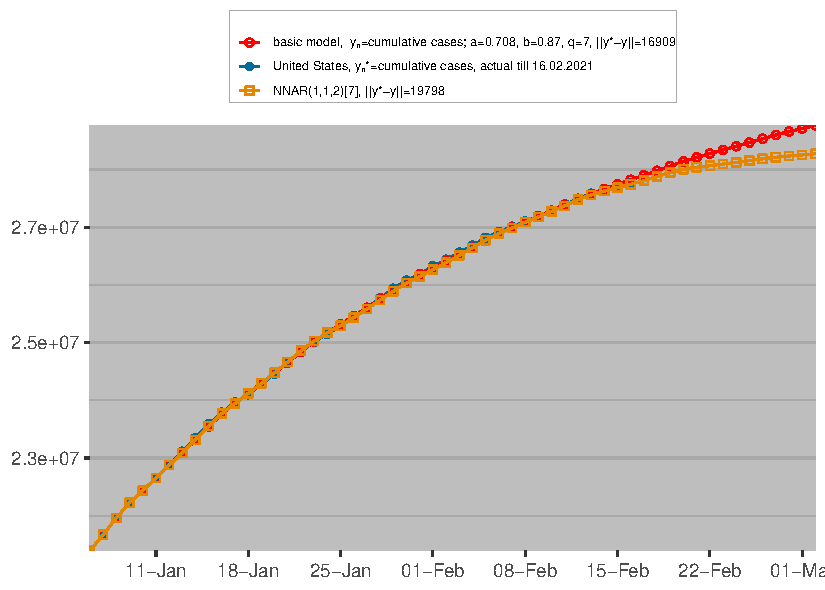
\includegraphics[width=0.9\textwidth]{Plots/United States-nny.pdf}
\end{figure}
\end{frame}

\begin{frame}{Ireland - Overfitting the Neural Network Model}
\begin{figure}
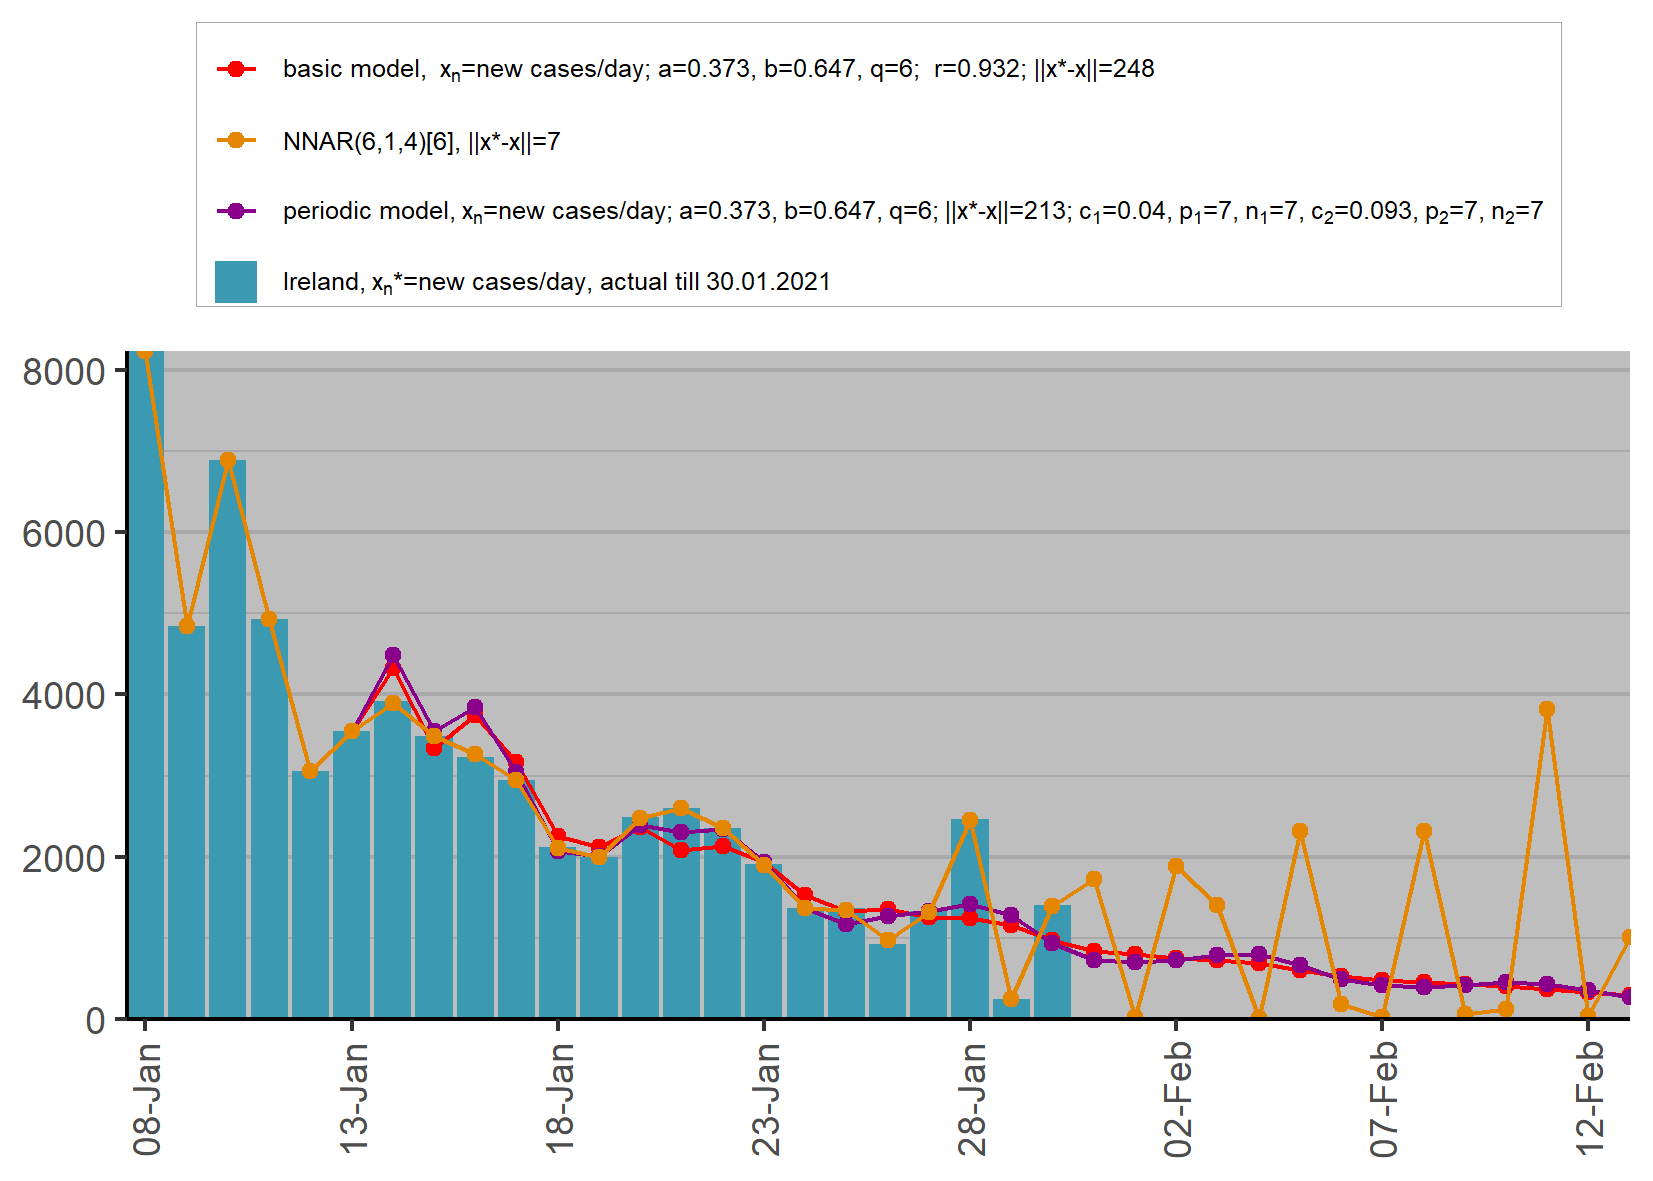
\includegraphics[width=0.9\textwidth]{Plots/Ireland-overfit.png}
\end{figure}
\end{frame}

\begin{frame}{Future work}
    \begin{itemize}
        \item Improve optimisation algorithm (danger of local optima, like with Ireland below)
    \end{itemize}
    \begin{figure}
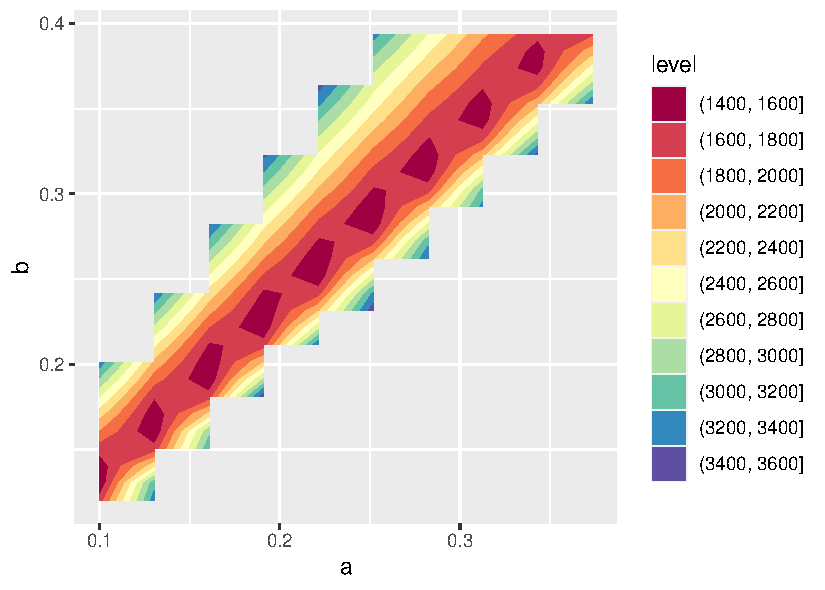
\includegraphics[width=0.9\textwidth]{Plots/Ireland-zoomcontour.pdf}
\end{figure}
\end{frame}

\begin{frame}{Future work}
    What's left to do:
    \begin{itemize}
        \item \textbf{Train} and \textbf{Test} datasets to rigorously compare models.
        \item Factor in distance $\left|\left|y^*-y\right|\right|$ to ensure the basic model matches \textbf{cumulative cases} as well as daily cases
        \item Improving code \textbf{efficiency}
    \end{itemize}
\end{frame}

\begin{frame}{References}
    \printbibliography
\end{frame}

\end{document}
